\documentclass[usenames,dvipsnames,notes]{beamer}
\usepackage{ifthen}
\usepackage{xcolor}
\usepackage{pgfplots}
\usepackage{amsmath}
\usepackage{centernot}
\usepackage{pifont}
\usepackage{tabularx}
\usepackage{makecell}
\usepackage{cuted}
\usepackage{booktabs}
\usepackage{array}

\usepackage{pgfpages}
%\setbeameroption{show notes on second screen}


\input ../beamer-style
\input ../std-macros
\input ../macros

\AtBeginSection[]
{
    \begin{frame}
        \frametitle{Table of Contents}
        \tableofcontents[currentsection]
    \end{frame}
}
\parskip=10pt

\title[CSCI-GA.2590]{Language Models}
\author[He He]{He He
}
\institute[NYU]{New York University}
\date{\today}

\begin{document}
\begin{frame}
\titlepage
\end{frame}

\section{Introduction}

\begin{frame}
    {Predict sequences}
    First part:\\
    \begin{itemize}
        \item Text representation $\phi\colon \text{text} \rightarrow \BR^d$
            \begin{itemize}
                \item BoW representation
                \item Distributed representation (word embeddings)
            \end{itemize}
        \item Probabilistic models
            \begin{itemize}
                \item Multinomial Naive Bayes
                \item Logistic regression
            \end{itemize}
    \end{itemize}

    Second part:\\
    \begin{itemize}
        \item Predict sequences
        \item Predict trees
        \item Inference algorithms
    \end{itemize}
\end{frame}

\begin{frame}
    {Language modeling}
    \emph{Motivation}: pick the most probable sentence
    \begin{itemize}
        \item Speech recognition
            \begin{itemize}
                \item[] the \textit{tail} of a dog
                \item[] the \textit{tale} of a dog
            \end{itemize}
            \begin{itemize}
                \item[] It's not easy to \textit{wreck a nice beach}. 
                \item[] It's not easy to \textit{recognize speech}. 
                \item[] It's not easy to \textit{wreck an ice beach}.
            \end{itemize}
        \item Machine translation 
            \begin{itemize}
                \item[] He sat on the \textit{table}.
                \item[] He sat on the \textit{figure}.
            \end{itemize}
            \begin{itemize}
                \item[] Such a Europe would \textit{the rejection of any} ethnic nationalism. 
                \item[] Such a Europe would \textit{mark the refusal of all} ethnic nationalism. 
            \end{itemize}
    \end{itemize}
\end{frame}

\begin{frame}
    {Problem formulation}
    \begin{itemize}
        \item \textbf{Vocabulary}: a \textit{finite} set of symbols $\sV$, e.g.\\
            \indent $\pc{\text{fox}, \text{green}, \text{red}, \text{dreamed}, \text{jumped}, \text{a}, \text{the}}$
        \item \textbf{Sentence}: a \textit{finite} sequence over the vocabulary $x_1 x_2 \ldots x_n \in \sV^n$ where $n\ge 0$ (empty sequence when $n=0$)
        \item The set of all sentences: $\sV^*$ 
        \item Goal: Assign a probability $p(x)$ to all sentences $x\in\sV^*$. 
    \end{itemize}

    \pause
    Assign probabilities:\\
    \begin{itemize}
        \item[] \text{the fox jumped}
        \item[] \text{the green fox dreamed}
        \item[] \text{the green dreamed fox}
        \item[] \text{dreamed red fox the}
    \end{itemize}
\end{frame}

\section{N-gram language models}

\begin{frame}
    {Learning a LM}
    \begin{itemize}
        \itemsep1em
        \item Given a corpus consisting of a set of sentences: $D=\pc{x^{(i)}}_{i=1}^N$
        \item Define
            $$
            p_s(x) = \frac{\text{count(x)}}{N} \;.
            $$
            (Check that $\sum_{x\in\sV^*}p_s(x) = 1$.)
        \item Is $p_s$ a good LM?
    \end{itemize}
    \vspace{4em}
    \pause
    Need to reduce the number of model parameters.
\end{frame}

\begin{frame}
    {Simplification 1: sentences to symbols}
    Decompose the joint probability using \textbf{chain rule}:
            \begin{align*}
            p(x) &= p(x_1, \ldots, x_n) \\
                &= p(x_1)p(x_2\mid x_1)p(x_3\mid x_1, x_2)\ldots p(x_n\mid x_{1}, \ldots, x_{n-1})
            \end{align*}

    \vspace{4em}
    Reduced number of outcomes: $\sV^*$ (sentences) to $\sV$ (symbols)

    But there is still a large number of contexts!
\end{frame}

\begin{frame}
    {Simplification 2: limited context}
    Reduce dependence on context by the \textbf{Markov assumption}:\\
    \begin{itemize}
        \item First-order Markov model
            \begin{align*}
                p(x_i\mid x_1,\ldots, x_{i-1}) &= p(x_i\mid x_{i-1}) \\
                p(x) &= \prod_{i=1}^n p(x_i\mid x_{i-1})
            \end{align*}
        \item Number of contexts: $|\sV|$
        \item Number of parameters: $|\sV|^2$
    \end{itemize}

    Beginning of a sequence:\\
    $$
    p(x_1\mid x_{1-1}) = ?
    $$
    Assume sequence starts with a special start symbol: $x_0=*$.
\end{frame}

\begin{frame}
    {Model sequences of variable lengths}
    Sample a sequence from the first-order Markov model $p(x_i\mid x_{i-1})$:\\
    \vspace{3em}

    When to stop?

    \pause
    Assume that all sequences end with a stop symbol \texttt{STOP}, e.g.
    \begin{align*}
        &\quad p(\text{the}, \text{fox}, \text{jumped}, \texttt{STOP})\\
         &= p(\text{the}\mid {\color{blue}*})
         p(\text{fox}\mid \text{the})
         p(\text{jumped}\mid \text{fox})
         p({\color{blue}\texttt{STOP}}\mid \text{jumped})
    \end{align*}

    LM with the \texttt{STOP} symbol:\\
    \begin{itemize}
        \item Vocabulary: $\texttt{STOP} \in \sV$
        \item Sentence: $x_1 x_2 \ldots x_n \in \sV^n$ for $n\ge 1$ and $x_n=\texttt{STOP}$.
    \end{itemize}
\end{frame}

\begin{frame}
    {N-gram LM}
    \begin{itemize}
        \item Unigram language model:
            $$
            p(x_1,\ldots, x_n) = \prod_{i=1}^n p(x_i) \;.
            $$
        \item Bigram language model ($x_0=*$):
            $$
            p(x_1,\ldots, x_n) = \prod_{i=1}^n p(x_i\mid x_{i-1}) \;.
            $$
        \item Trigram language model ($x_{-1}=*,x_0=*$):
            $$
            p(x_1,\ldots, x_n) = \prod_{i=1}^n p(x_i\mid x_{i-2}, x_{i-1}) \;.
            $$
        \item $n$-gram language model:
            $$
            p(x_1,\ldots, x_m) = \prod_{i=1}^m p(x_i\mid \underbrace{
                x_{i-n+1},\ldots, x_{i-1}
            }_{\text{previous $n-1$ words}} )
            \;.
            $$
    \end{itemize}
\end{frame}

\begin{frame}
    {Parameter estimation}
    \begin{itemize}
        \itemsep1em
        \item Data: a corpus $\pc{x^{(i)}}_{i=1}^N$ where $x\in\sV^n$.
        \item Model: bigram LM $p(w\mid w')$ for $w,w'\in\sV$.
            $$
            p(w\mid w') = \theta_{w\mid w'}
            $$
            where $\sum_{w\in\sV}p(w\mid w') = 1 \quad \forall w'\in\sV$.
    \end{itemize}

    MLE:
    \vspace{5em}
\end{frame}

\begin{frame}
    {MLE solution}
    \begin{itemize}
        \itemsep1em
        \item Unigram LM
            $$
            \hat{p}(x) = \frac{\text{count}(w)}{\sum_{w\in\sV}\text{count}(w)}
            $$
        \item Bigram LM
            $$
            \hat{p}(w\mid w') =
            \frac{\text{count}(w,w')}{\sum_{w\in\sV}\text{count}(w,w')}
            $$
        \item In general, for n-gram LM,
            $$
            \hat{p}(w\mid c) =
            \frac{\text{count}(w,c)}{\sum_{w\in\sV}\text{count}(w,c)}
            $$
            where $c\in \sV^{n-1}$.
    \end{itemize}
\end{frame}

\begin{frame}
    {Example}
    \begin{itemize}
        \item Training corpus
            \begin{itemize}
                \item[] $\pc{\text{The fox is red},
                    \text{The red fox jumped},
                    \text{I saw a red fox}
                    }$
            \end{itemize}
        \item Collect counts
            \begin{itemize}
                \item[] $\text{count}(\text{fox})=3$
                \item[] $\text{count}(\text{red})=3$
                \item[] $\text{count}(\text{red}, \text{fox})=2$
                \item[] $\ldots$
            \end{itemize}
        \item Parameter estimates
            \begin{itemize}
                \item[] $\hat{p}(\text{red}\mid\text{fox})=$
                \item[] $\hat{p}(\text{saw}\mid\text{i})=$
            \end{itemize}
        \pause
        \item What is the probability of ``I saw a brown fox jumped''?
    \end{itemize}
\end{frame}

\begin{frame}
    {Real n-gram counts}
    Google Books n-gram counts
    \begin{figure}
        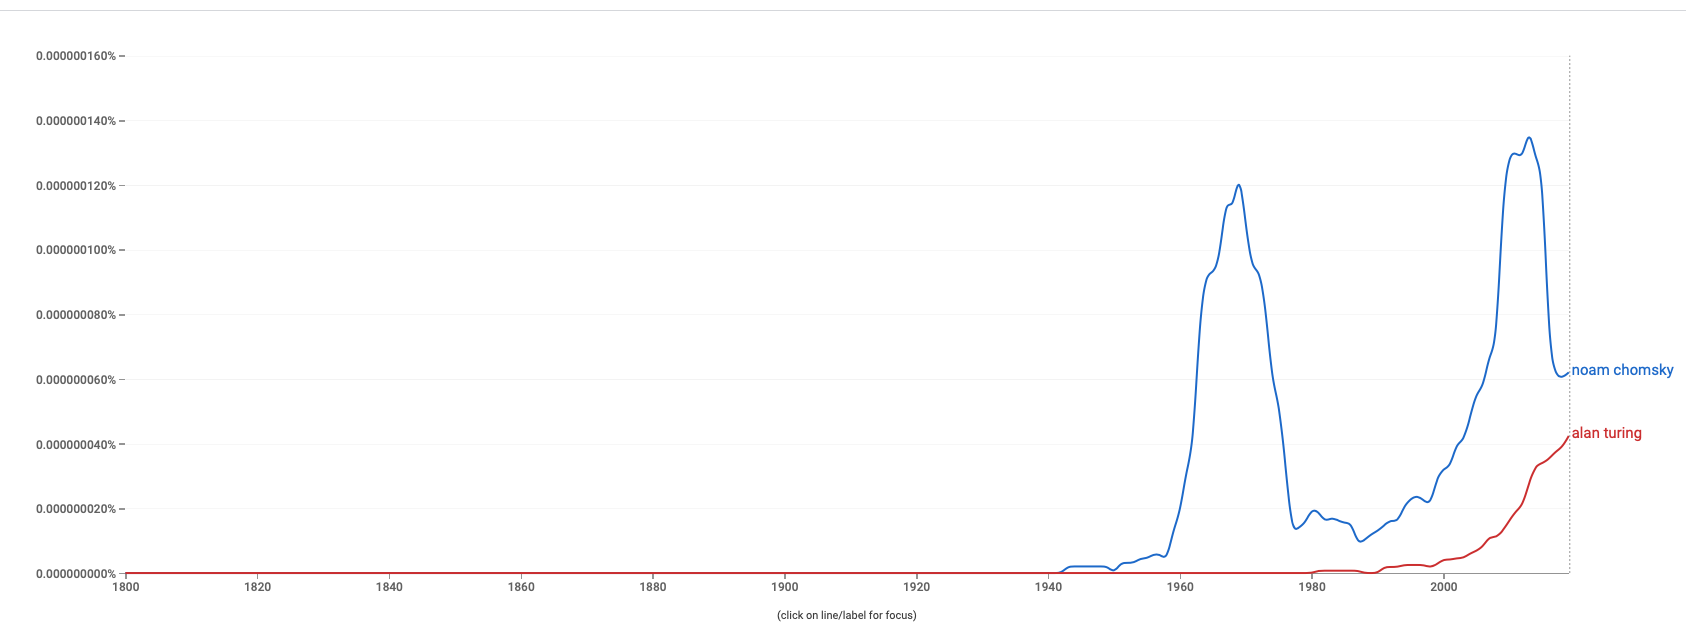
\includegraphics[height=3cm]{figures/google-ngram}
    \end{figure}

    Efficient implementation\\
    \begin{itemize}
        \item Memory, inference speed
        \item Context encodings, tries, caching, ...
        \item \texttt{kenlm} (\url{https://github.com/kpu/kenlm})
    \end{itemize}
\end{frame}

\begin{frame}
    {Summary}
    \textbf{Language models}: assign probabilities to sentences

    \textbf{N-gram language models}:\\
    \begin{itemize}
        \item Assume each word only conditions on the previous $n-1$ words
        \item MLE estimate: counting n-grams in the training corpus
    \end{itemize}

    Problems with vanilla n-gram models:\\
    \begin{itemize}
        \item Estimate of probabilities involving rare n-grams is inaccurate
        \item Sentences containing unseen n-grams have zero probability
    \end{itemize}
\end{frame}

\begin{frame}
    {Backoff and interpolation}
    What context size should we use?

    \textbf{Backoff}:
    Use higher-order models when we have enough evidence.
    \begin{itemize}
        \item Stupid backoff:
    $$
    \hat{p}(x_i\mid x_{i-n+1:i-1}) = \begin{cases}
        \frac{\text{count}(x_{i-n+1:i})}{\text{count}(x_{i-n+1:i-1})} & \text{if } \text{count}(x_{i-n+1:i}) > 0 \\
        \lambda \hat{p}(x_i\mid x_{i-n+2:i-1}) & \text{otherwise}
    \end{cases}
    $$
    \end{itemize}


    \textbf{Interpolation}: mixture of n-gram models
    $$
    p(x_i\mid x_{i-2}, x_{i-1}) = \lambda_1 p(x_i\mid x_{i-2}, x_{i-1})
    + \lambda_2 p(x_i\mid x_{i-1})
    + \lambda_3 p(x_i)
    $$
    where $\lambda_1 + \lambda_2 + \lambda_3=1$.
    \begin{itemize}
        \item $\lambda$ can depend on context.
        \item Tune $\lambda$'s on the validation set.
    \end{itemize}
\end{frame}

\begin{frame}
    {Smoothing}
    How to estimate frequencies of unseen words?

    More generally, estimate unseen elements in the support of a distribution.\\
    \begin{itemize}
        \item Given frequencies of observed species, what's the probability of encountering a new species?
        \item Given observed genetic variations from a certain population, what's the probability of observing new mutations?
    \end{itemize}

    \emph{Key idea}: reserve some probability mass for unseen words
    \vspace{6em}
\end{frame}

\begin{frame}
    {Add-$\alpha$ smoothing}
    Original estimate: \\
    \vspace{2em}

    Smoothed estiamte:\\ 
    \vspace{2em}

    Discounted counts:\\
    \vspace{4em}
\end{frame}

\begin{frame}
    {Add-one smoothing}
    How does smoothing change the estimate?

    Example:\\
    \begin{itemize}
        \item[] $\text{count}(x)=10, N=100, |\sV|=1000$
        \item[] Original: $10/100=0.1$
        \item[] Smoothed: $(10+1)/(100+1000)\approx 0.01$
    \end{itemize}

    Assigns too much probability mass to unseen words!

    Tuning $\alpha$ on validation set helps but still not good enough for LM.
\end{frame}

\begin{frame}
    {Good-Turing smoothing}
    \emph{Key idea}: use the validation set for estimation\\
    \vspace{5em}

    Leave-one-out cross validation\\
    \vspace{8em}

\end{frame}

\begin{frame}
    {Good-Turing smoothing}
    \begin{itemize}
        \item Let $N_r$ be the number of tokens that occur $r$ times in the corpus
        \item How many held-out tokens are unseen during training? 
            \vspace{2em}
        \item How many held-out tokens are seen $k$ times during training? 
            \vspace{2em}
        \item What's the ``correct'' count of a word that occur $k$ times in the corpus?
            \vspace{2em}
        \item What's the probability of a word that occur $k$ times in training?
            \vspace{2em}
    \end{itemize}
\end{frame}

\begin{frame}
    {Kneser-Ney smoothing}
    Widely used for n-gram LMs.

    \emph{Idea 1}: absolute discounting.
    \begin{figure}
        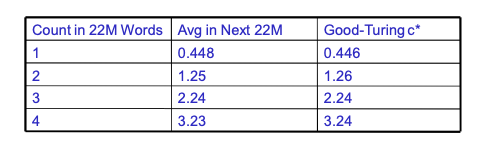
\includegraphics[height=2.5cm]{figures/good-turing}
        \caption{Good-Turing counts from Dan Klein's slides}
    \end{figure}

    Just subtract 0.75 or some constant.
\end{frame}

\begin{frame}
    {Kneser-Ney smoothing}
    \emph{Idea 2}: consider word \emph{versatility} rather than word counts.

    \emph{Motivation}:\\
    \begin{itemize}
        \item[] $\text{count}(\text{San Francisco})=100$, $\text{count}(\text{Minneapolis})=10$
        \item[] I recently visited $\rule{1cm}{0.15mm}$.
    \end{itemize}
    \pause
    Some words can only follow specific contexts, i.e. less versatile.

    \textbf{Continuation probability}: how likely is $w$ allowed in a context\\
    \begin{itemize}
        \item[] $p_{\text{unigram}}(w) \propto \sum_{w'\in\sV}\text{count}(w, w')$
        \item[] $p_{\text{continuation}}(w) \propto |\pc{w'\colon \text{count}(w, w') > 0}|$
        \item[] $$\beta(w) = \frac{\text{\# bigram types ends with $w$}}{\text{\# bigram types}}$$
    \end{itemize}
\end{frame}

\begin{frame}
    {Kneser-Ney smoothing}
    Combine the two ideas:

    $$
    \hat{p}(w\mid w') = \frac{\text{count}(w, w') - d}{\text{count(w')}} + \lambda(w')p_{\text{continuation}}(w)
    $$
    \vspace{2em}

    \begin{itemize}
        \item Works well for ASR and MT.
        \item Dominating n-gram model before neural LMs.
    \end{itemize}
\end{frame}

\begin{frame}
    {Summary}
    Key ideas in n-gram language models:

    \textbf{Markov assumption}:\\
    \begin{itemize}
        \item Trigram models are reasonable.
        \item ASR, MT often use 4- or 5-gram models.
    \end{itemize}

    \textbf{Discounting / Smoothing}:\\
    \begin{itemize}
        \item ``Borrow'' probability mass for unseen words
        \item Good-Turing smoothing, absolute discount
    \end{itemize}

    \textbf{Dynamic context}:\\
    \begin{itemize}
        \item Use more context if there is evidence
        \item Katz backoff, Kneser-Ney
    \end{itemize}

    See Chen and Goodman (1999) for more results.
\end{frame}

\section{Neural language models}
\begin{frame}
    {N-gram models by classification}
    \textbf{Log-linear} language model:
    $$
    p(w\mid c) = \frac{
        \exp\pb{\theta\cdot \phi(w, c)}
    }{
        \sum_{w'\in\sV}\exp\pb{\theta\cdot \phi(w', c)}
    }
    $$

    Feature templates:\\
    \vspace{9em}

    Learn by MLE and SGD.
\end{frame}

\begin{frame}
    {Feed-forward neural networks}
    Key idea in neural nets: feature/representation learning 

    Building blocks:\\
    \begin{itemize}
        \itemsep2em
        \item Input layer: raw features (no learnable parameters)
        \item Hidden layer: perceptron + nonlinear activation function
        \item Output layer: linear (+ transformation, e.g. softmax)
    \end{itemize}
\end{frame}

\begin{frame}
    {Feed-forward neural language models}
    Encode the (fixed-length) context using feed-forward NN:
    \begin{figure}
        \includegraphics[height=5cm]{figures/fflm}
    \end{figure}
\end{frame}

\begin{frame}
{Computation graphs}
Function as a \emph{node} that takes in \emph{inputs} and produces \emph{outputs}.

\begin{columns}[t]
\column{.5\textwidth}
\begin{itemize}
\item Typical computation graph:
\end{itemize}
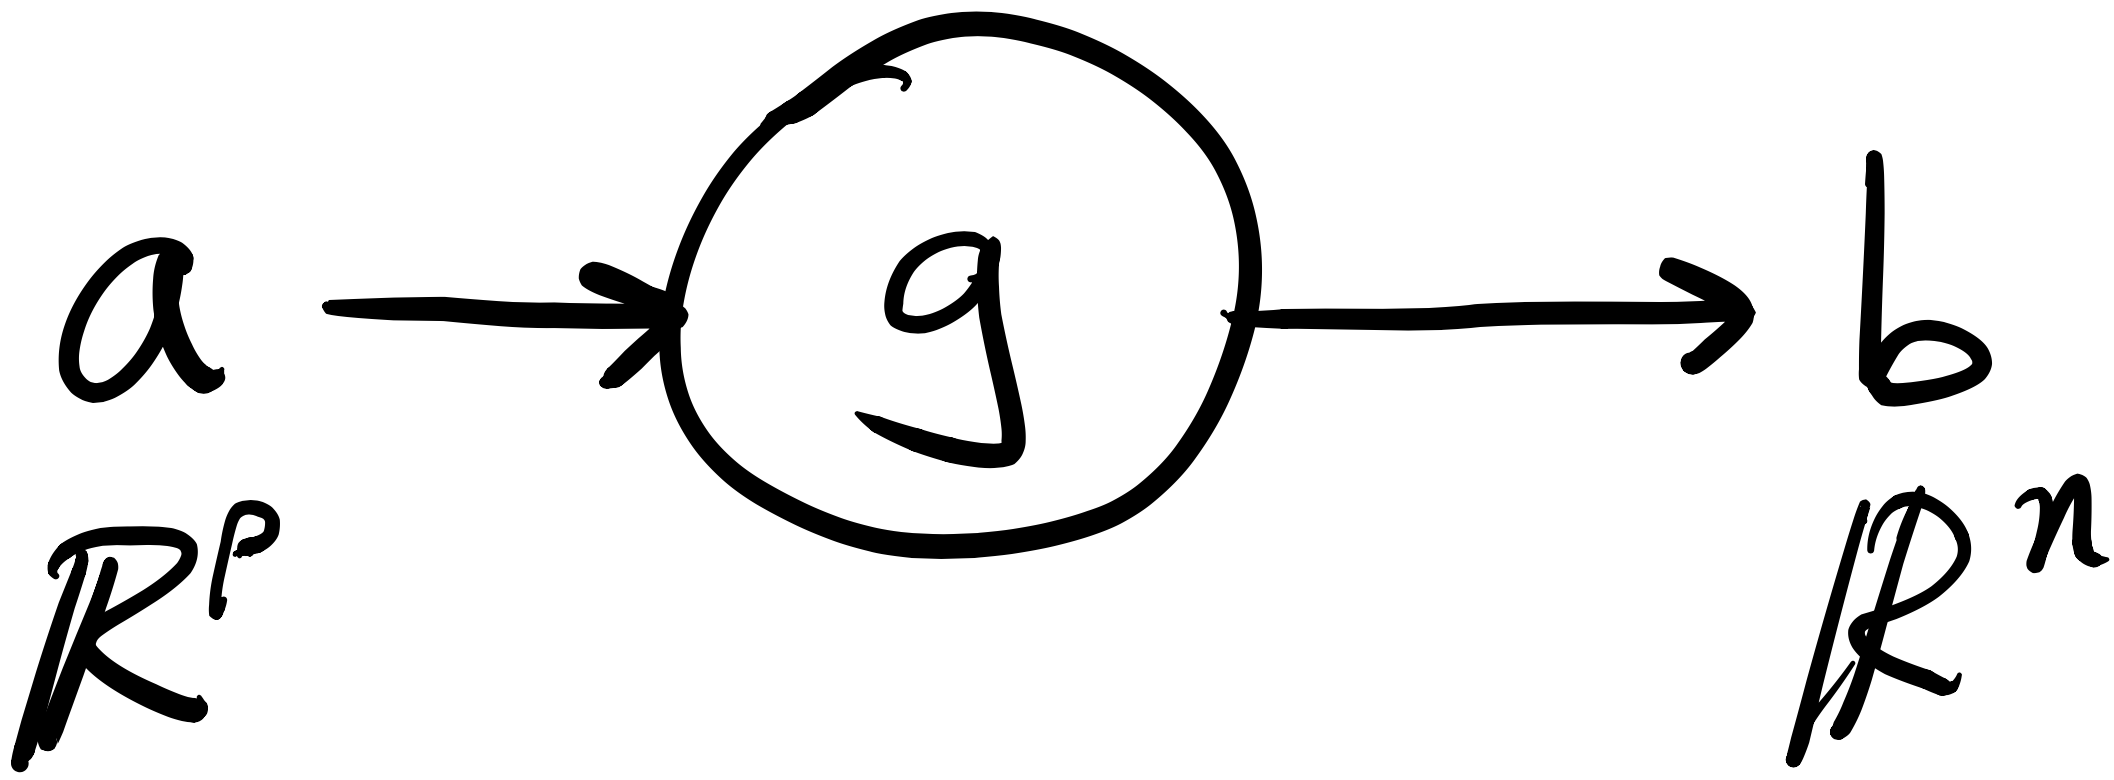
\includegraphics[scale=0.05]{figures/one-fn-comp-graph}

\column{.5\textwidth}
\begin{itemize}
\item Broken out into components:
\end{itemize}
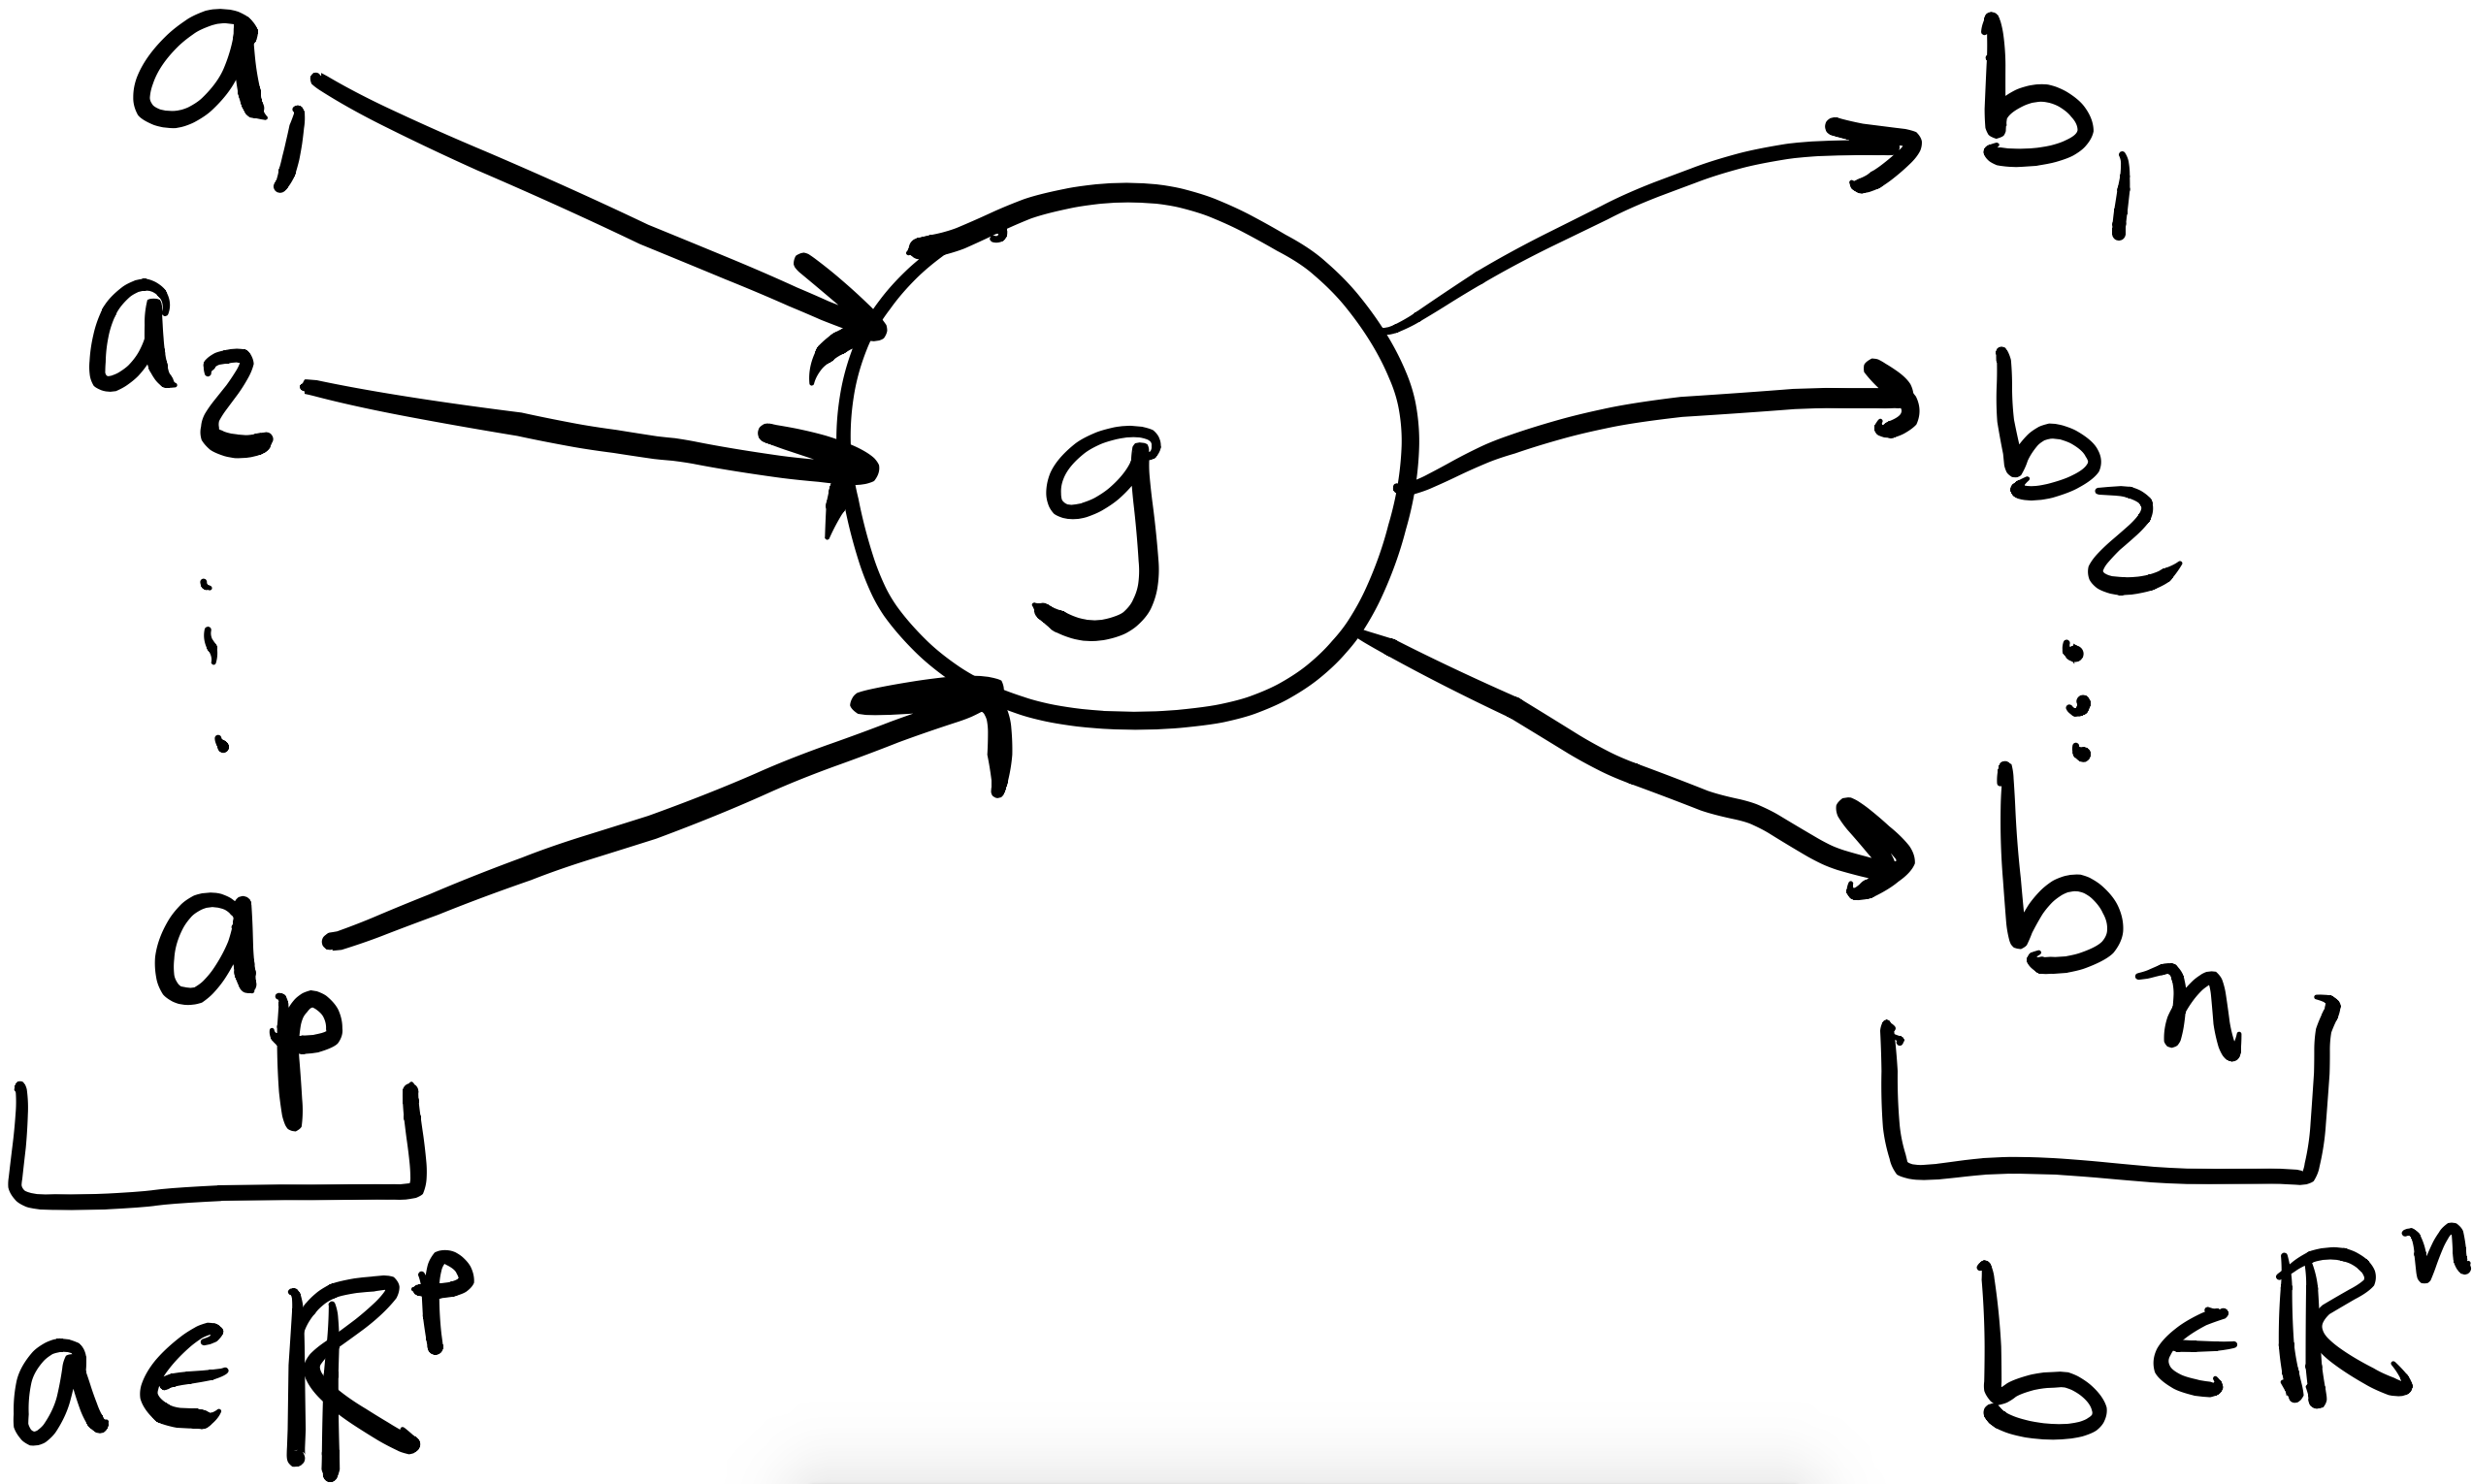
\includegraphics[scale=0.05]{figures/one-fn-comp-graph-partials}
\end{columns}
\end{frame}

\begin{frame}
{Compose multiple functions}
Compose two functions $g:\BR^{p}\to\BR^{n}$ and $f:\BR^{n}\to\BR^{m}$.
\begin{figure}
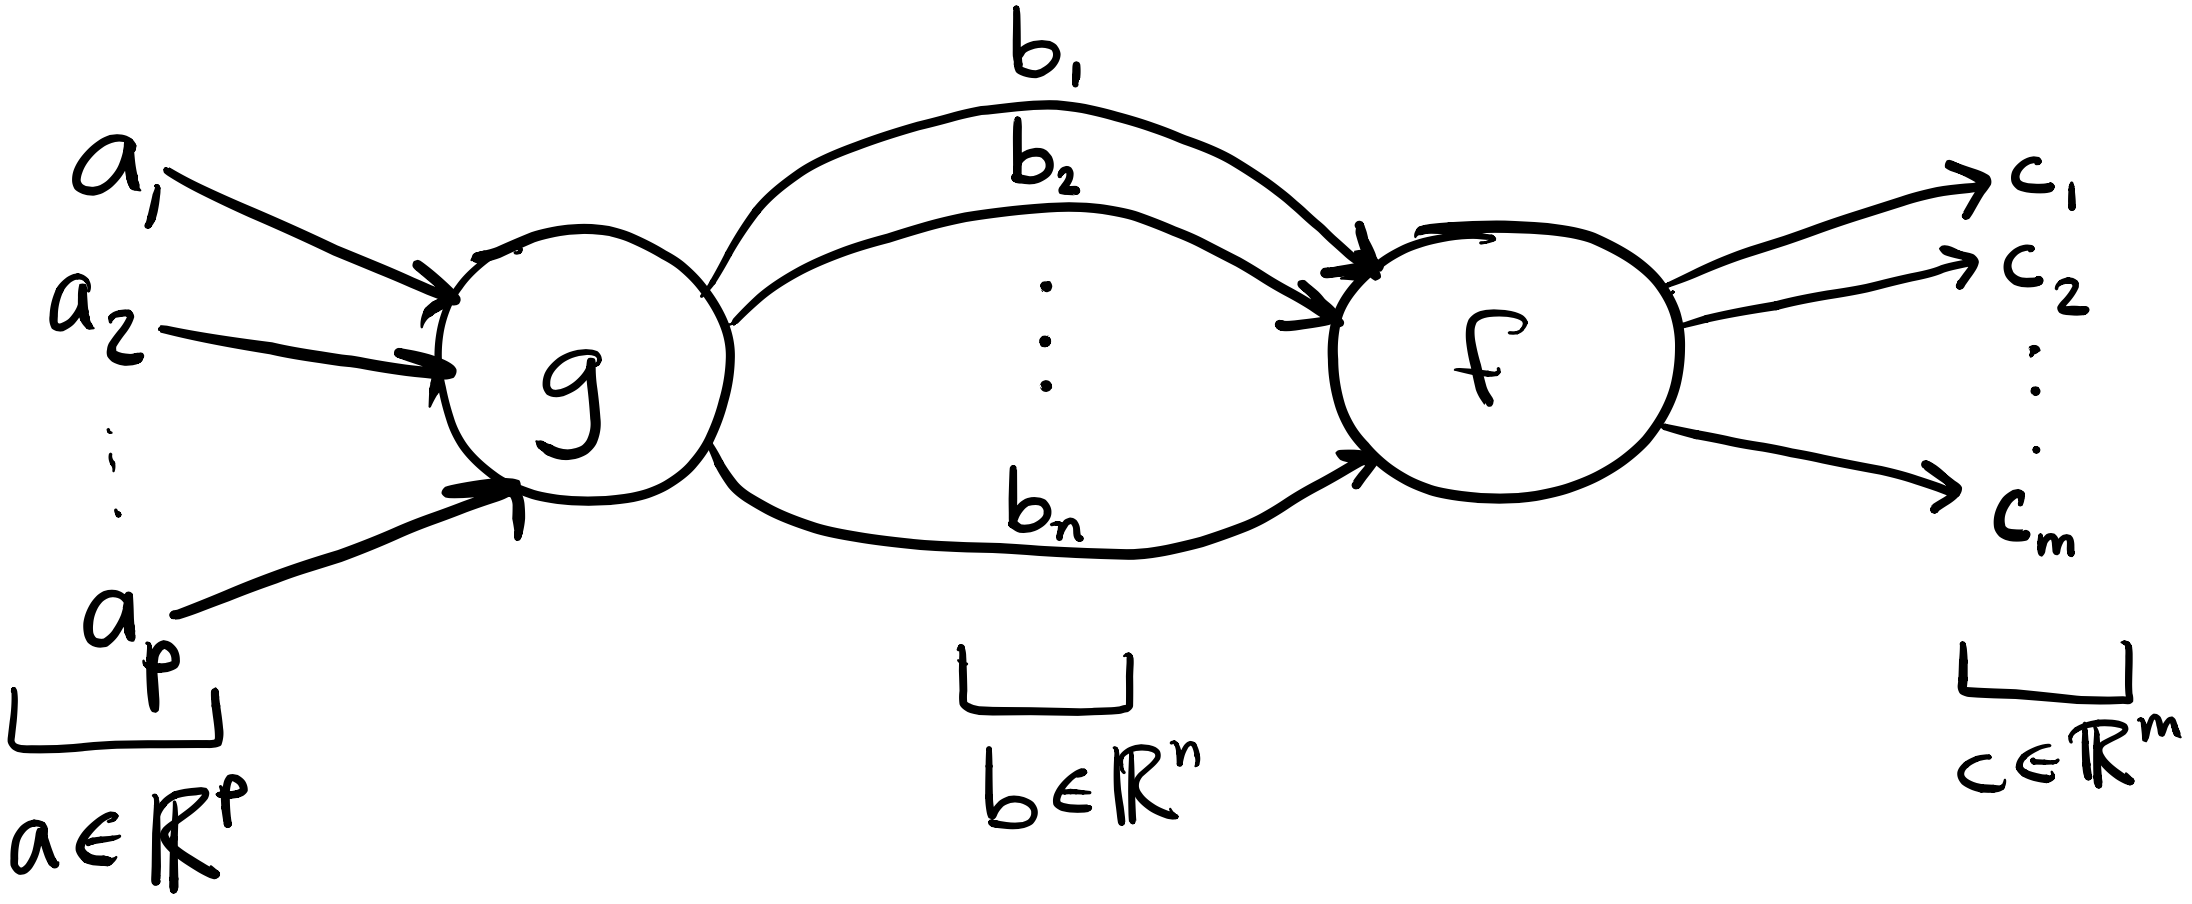
\includegraphics[height=2.5cm]{figures/two-fn-comp-graph-partials}
\end{figure}

\begin{itemize}
\item How does change in $a_j$ affect $c_i$?
\item Visualize \textbf{chain rule}:
\begin{itemize}
\item \textcolor{blue}{Sum} changes induced on all paths from $a_j$ to $c_i$.
\item Changes on one path is the {\color{red}product} of changes on each edge.
\[
\frac{\partial c_{i}}{\partial a_{j}}={\color{blue}\sum_{k=1}^{n}}
{\color{red} \frac{\partial c_{i}}{\partial b_{k}}\frac{\partial b_{k}}{\partial a_{j}}} .
\]
\end{itemize} 
\end{itemize}
\end{frame}

\begin{frame}
    {Computation graph example}
\end{frame}

\begin{frame}
    {Backpropogation}
    Backpropogation = chain rule + dynamic programming on a computation graph

    Forward pass
\begin{itemize}
\item \textbf{Topological order}: every node appears before its children
\item For each node, compute the output given the input (from its parents).
\end{itemize}
\begin{center}
\begin{tikzpicture}[shorten >=1pt]
      	\tikzstyle{unit}=[draw,shape=circle,minimum size =1cm]

		\node (start) at (0,1){$\ldots$};
       	\node[unit](i) at (3,1){$f_i$};
        	\node[unit](j) at (6,1){$f_j$};
        	\node (end) at (9,1){$\ldots$};

        	\draw[->] (i) -- (j);
        	\draw[->] (start) -- (i);
        	\draw[->] (j) -- (end);
		
		\begin{scope}[transform canvas={yshift=-.7em}]
		\draw [->, Green, line width=0.05cm, shorten <=1mm, shorten >=1mm] (start) -- node {} (i);
  		\draw [->, Green, line width=0.05cm, shorten <=1mm, shorten >=1mm] (i) -- node {} (j);
  		\draw [->, Green, line width=0.05cm, shorten <=1mm, shorten >=1mm] (j) -- node {} (end);
		\end{scope}
		
		\begin{scope}[transform canvas={yshift=-1.4em}]
		\node (i-in) [right=0.2cm of start] {$a$};
		\node (j-in) [right=0.2cm of i] {$b=f_i(a)$};
		\node (j-out) [right=0.2cm of j] {$c=f_j(b)$};
		\end{scope}
\end{tikzpicture}
\end{center}
    \vspace{3em}
\end{frame}

\begin{frame}
    {Backpropogation}
    Backward pass
\begin{itemize}
\item \textbf{Reverse topological order}: every node appear after its children
\item For each node, compute the partial derivative of its output w.r.t. its input, multiplied by the partial derivative from its children (chain rule).
\end{itemize}
\begin{center}
\begin{tikzpicture}[shorten >=1pt]
      	\tikzstyle{unit}=[draw,shape=circle,minimum size =1cm]

		\node (start) at (0,1){$\ldots$};
       	\node[unit](i) at (3,1){$f_i$};
        	\node[unit](j) at (6,1){$f_j$};
        	\node (end) at (9,1){$\ldots$};

        	\draw[->] (i) -- (j);
        	\draw[->] (start) -- (i);
        	\draw[->] (j) -- (end);
		
		\begin{scope}[transform canvas={yshift=-.7em}]
		\draw [->, Green, line width=0.05cm, shorten <=1mm, shorten >=1mm] (start) -- node {} (i);
  		\draw [->, Green, line width=0.05cm, shorten <=1mm, shorten >=1mm] (i) -- node {} (j);
  		\draw [->, Green, line width=0.05cm, shorten <=1mm, shorten >=1mm] (j) -- node {} (end);
		\end{scope}
		
		\begin{scope}[transform canvas={yshift=-1.4em}]
		\node (i-in) [right=0.2cm of start] {$a$};
		\node (j-in) [right=0.2cm of i] {$b=f_i(a)$};
		\node (j-out) [right=0.2cm of j] {$c=f_j(b)$};
		\end{scope}
		
		\begin{scope}[transform canvas={yshift=-2.5em}]
		\draw [<-, red, line width=0.05cm, shorten <=1mm, shorten >=1mm] (start) -- node {} (i);
  		\draw [<-, red, line width=0.05cm, shorten <=1mm, shorten >=1mm] (i) -- node {} (j);
%  		\draw [<-, red, line width=0.05cm, shorten <=1mm, shorten >=1mm] (j) -- node {} (end);
		\end{scope}
		
		\begin{scope}[transform canvas={yshift=-3.4em}]
		\node (i-out) [left=0.2cm of i] {$g_i=g_j \cdot \frac{\partial b}{\partial a} = \frac{\partial J}{\partial a}$};
		\node (j-out) [left=0.2cm of j] {$g_j=\frac{\partial J}{\partial b}$};
		\end{scope}
\end{tikzpicture}
\end{center}
    \vspace{3em}
\end{frame}

\begin{frame}
    {Summary}
    Neural networks\\
    \begin{itemize}
        \item Automatically learn the features
        \item Optimize by SGD (implemented by back-propogation)
        \item Non-convex, may not reach a global minimum
    \end{itemize}

    Feed-forward neural language models\\
    \begin{itemize}
        \item Use fixed-size context (similar to n-gram models)
        \item Represent context by feed-forward neural networks
    \end{itemize}
\end{frame}

\section{Recurrent Neural Networks}

\begin{frame}
    {Recurrent neural networks}
    How much context is needed?\\
    ... I went $\rule{1cm}{0.15mm}$ $\rule{1cm}{0.15mm}$

    Idea: compute context representation recurrently
    $$
 h_t = \sigma(\underbrace{W_{hh}h_{t-1}}_{\text{previous state}}+
 \underbrace{W_{ih}x_t}_{\text{new input}} + b_h)
 \;.
    $$

    \begin{figure}
        \includegraphics[height=3cm]{figures/rnn}
    \end{figure}
\end{frame}

\begin{frame}
    {Backpropogation through time}
    Exercise: compute $\frac{\partial h_t}{\partial h_i}$
    $$
 h_t = \sigma(\underbrace{W_{hh}h_{t-1}}_{\text{previous state}}+
 \underbrace{W_{ih}x_t}_{\text{new input}} + b_h)
 \;.
    $$

    Problem:\\
    \begin{itemize}
        \item Gradient involves repeated multiplication of $W_{hh}$
        \item Gradient will vanish / explode
    \end{itemize}

    Quick fixes:\\
    \begin{itemize}
        \item Truncate after $k$ steps (i.e. \texttt{detach} in the backward pass)
        \item Gradient clipping
    \end{itemize}
\end{frame}

\begin{frame}
    {Gated recurrent neural networks}
    %\emph{Key idea}: have a separate mechanism to decide when to ``memorize'' or ``forget'' a state

    Long-short term memory (LSTM)\\
    \begin{itemize}
        \item \emph{Memory cell}: decide when to ``memorize'' or ``forget'' a state
            \begin{align*}
                c_t &= \underbrace{i_t \odot \tilde{c}_t}_{\text{update with new memory}} +
     \underbrace{f_t \odot c_{t-1}}_{\text{reset old memory}}\\
                \tilde{c}_t &= \tanh(W_{xc}x_t + W_{hc}h_{t-1} + b_c) \;.
            \end{align*}

            \item Input gate and forget gate
            \begin{align*}
 i_t &= \text{sigmoid}(W_{xi}x_t + W_{hi}h_{t-1} + b_i) \;,\\
 f_t &= \text{sigmoid}(W_{xf}x_t + W_{hf}h_{t-1} + b_f) \;.
            \end{align*}

            \item Hidden state
            \begin{align*}
 h_t &= o_t \odot c_t \;\text{, where} \\
 o_t &= \text{sigmoid}(W_{xo}x_t + W_{ho}h_{t-1} + b_o) \;.
            \end{align*}
    \end{itemize}
\end{frame}

\section{Evaluation}
\begin{frame}
    {Perplexity}
    What is the loss function for learning language models?

    Held-out likelihood on test data $D$:
    $$
    \ell({D}) = \sum_{i=1}^{|D|} \log p_\theta(x_i\mid x_{1:i-1}) \;,
    $$

    \textbf{Perplexity}:
    $$
 \text{PPL}(D) = 2^{-\frac{\ell(D)}{|D|}} \;.
 $$
    \begin{itemize}
        \item Base of log and exponentiation should match
        \item Exponent is cross entropy: $H(p, p_\theta) = -\BE_{x\sim p}\log p_\theta(x)$.
        \item Interpretation: a model of perplexity $k$ predicts the next word by throwing a fair $k$-sided die.
    \end{itemize}
\end{frame}

\end{document}
